\documentclass[a4paper,12pt]{article}
\usepackage[utf8]{inputenc}
\usepackage{amsmath}
\usepackage{graphicx}
\usepackage{hyperref}
\usepackage{geometry}
\geometry{margin=1in}

\title{IR Transmission Research for Multi-Transmitter Systems}
\author{}
\date{}

\begin{document}

\maketitle

\section{Introduction}

While creating the NEC parallel transmitter, I encountered an interference problem when two transmitters are placed near each other. Therefore, I need to develop protection against this interference, such as a guiding tube or other isolation methods.

\section{Signal Characteristics}

My signal follows the NEC standard with a carrier frequency of \textbf{38 kHz}, and the wavelength of the transmission LED is \textbf{940 nm}~\cite{arduino}, which places it in the \textbf{NIR (Near-Infrared)} region.

\begin{figure}[h]
\centering
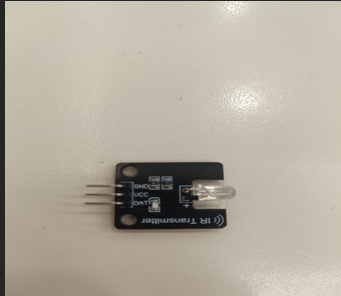
\includegraphics[width=0.4\textwidth]{img/Transmitter.png}
\caption{IR Transmitter Element}
\end{figure}

The spectral regions are illustrated in Figure~\ref{fig:regions}.

\begin{figure}[h]
\centering
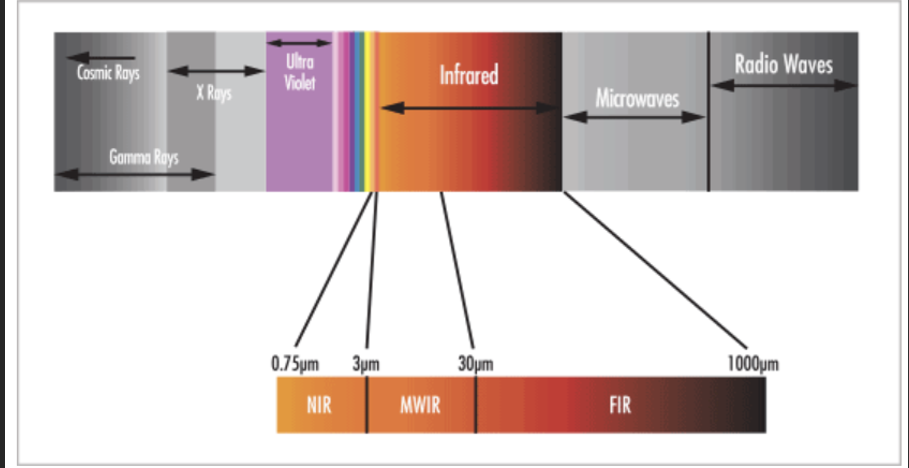
\includegraphics[width=0.8\textwidth]{img/NIR.png}
\caption{Infrared Spectral Regions~\cite{edmund}}
\label{fig:regions}
\end{figure}

\section{Physical Isolation Using Reflective Materials}

I searched for materials that reflect IR light to prevent interference between transmitters. Polished metals are commonly used for this purpose~\cite{carbodiimide}. I used copper metal, and it works properly for insulation.

\section{System Expansion}

I was asked to add more parallel transmitters. The maximum number of pins available for transmission is:
\begin{itemize}
    \item 8 pins from PMOD A
    \item 8 pins from PMOD B
    \item 20 pins from Arduino
\end{itemize}
This gives a total of \textbf{36 pins} for transmission. I will use 24 transmitters: all Arduino pins and 4 PMOD A pins.

\section{Frequency-Division Approach}

Physical barriers are not feasible, so alternative methods for IR transmission must be implemented. The proposed approach is \textbf{carrier frequency shifting} from 38 kHz to higher frequencies.

\subsection{Initial Plan}
The initial plan was to shift from \textbf{38 kHz to 84 kHz} with \textbf{2 kHz steps}. However, both the transmitter and receiver are designed for 38 kHz operation.

\subsection{Revised Frequency Plan}
Based on research, IR receivers can detect signals near their center frequency. To ensure sufficient separation, a \textbf{10 kHz spacing} is required. Therefore, the new frequency range is from \textbf{38 kHz to 278 kHz}.
This can be approached if we will use the TSAL6100 IR LED transmitter with different carrier frequency, we will do it using FPGA.

\subsection{Receiver Characteristics}
The main characteristics of the IR transmitter:
\begin{itemize}
    \item Range: 1.3 m (at 5V and 38 kHz)
    \item Wavelength: 940 nm
    \item Carrier frequency: 38 kHz (fixed for standard modules)
    \item Also possible to receive from 35KHZ to 41KHZ
\end{itemize}

\section{Alternative Approaches}
Other complex methods exist, such as channel reuse strategies for indoor infrared wireless communications~\cite{IEEE}.



\begin{thebibliography}{9}

\bibitem{medium}
Medium. \emph{NEC Transmission Protocol for Air Conditioners}. \\
\url{https://medium.com/blueeast/nec-transmission-protocol-for-air-conditioners-67c8a698e633}

\bibitem{edmund}
Edmund Optics. \emph{The Correct Material for Infrared Applications}. \\
\url{https://www.edmundoptics.com/knowledge-center/application-notes/optics/the-correct-material-for-infrared-applications/}

\bibitem{arduino}
ArduinoModules.info. \emph{KY-005 Infrared Transmitter Sensor Module}. \\
\url{https://arduinomodules.info/ky-005-infrared-transmitter-sensor-module/}

\bibitem{carbodiimide}
Carbodiimide. \emph{Near-Infrared Absorbing Materials and Their Applications}. \\
\url{https://carbodiimide.com/near-infrared-absorbing-materials-and-their-applications/}

\bibitem{IEEE}
\emph{Channel Reuse Strategies for Indoor Infrared Wireless Communications}. IEEE. \\
\url{https://ieeexplore.ieee.org/stamp/stamp.jsp?tp=&arnumber=591910}

\bibitem{askelectronics}
Ask Electronics. \emph{IR Infrared Transmitter Module}. \\
\url{https://askelectronics.co.ke/product/1-10pcs-ir-infrared-transmitter-module-ir-digital-38khz-infrared-receiver-sensor-module-for-arduino-electronic-building-block/}

\end{thebibliography}

\end{document}